\section{A star of cold, non-interacting fermions}
\label{section: cold fermi star}

This section is based on~\autocite{glendenningCompactStarsNuclear2012,andersenIntroductionStatisticalMechanics2012,kapustaFiniteTemperatureFieldTheory2006}.

In this section, we will study a simple model of a star made up of non-interacting, cold neutrons.
This is one of the earliest models used to study neutron stars, the remenants of massive stars~\autocite{glendenningCompactStarsNuclear2012}.
For this model, we use results derived in \autoref{section: fermions}.



\subsection{Thermodynamics and the equation of state}

The total energy $U$ is related to the grand canonical free energy $F$ by a Legendre transformation,
%
\begin{equation}
    F(T, V, \mu) = U - T S - \mu Q, \quad \dd F = - S \dd T - p \dd V - Q \dd \mu.
\end{equation}
%
Here $T = {1}/{\beta}$ is temperature, and $S$ entropy,  $p$ pressure, and $V$ volume.
$Q$ is some conserved charge, in our case the number of particles minus antiparticles, and $\mu$ is the corresponding chemical potential.
These thermodynamic variables are related to the free energy by
%
\begin{equation}
    S = - \pdv{F}{T} = \beta^2 \pdv{F}{\beta}, \quad
    Q = - \pdv{F}{\mu}, \quad
    p = - \pdv{F}{V}.
\end{equation}
%
When the free energy can be written as $F = V \Eff$, where the free energy density $\Eff$ is independent of the volume $V$, then $\Eff = - p$ and
%
\begin{equation}
    \dd (V \Eff) = V \dd \Eff - p \dd V,
\end{equation}
%
allowing us to write
%
\begin{equation}
    \Eff(T, \mu) = u - Ts - \mu n, \quad
    \dd \Eff = -s \dd T - n \dd \mu,
\end{equation}
% 
where $s$ and $n$ are entropy and charge density, defined by
%
\begin{equation}
    s = - \pdv{\Eff}{T} = \beta^2 \pdv{\Eff}{\beta}, \quad
    n = - \pdv{\Eff}{\mu}.
\end{equation}
%
With this, we can write the energy density as~\autocite{andersenIntroductionStatisticalMechanics2012}
%
\begin{equation}
    u = \pdv{}{\beta} \left(\beta \Eff\right) + \mu n.
\end{equation}
%

We calculate the free energy density of non-interacting fermions in \autoref{section: fermions}, with the result \autoref{free energy fermions},
%
\begin{equation}
    \Eff = - 
    \frac{2}{\beta}\int \frac{\dd^3 p}{(2 \pi)^3} 
    \left[
        \beta \omega
        +
        \ln\left(1 + e^{-\beta(\omega - \mu)}\right)
        + 
        \ln\left(1 + e^{-\beta(\omega + \mu)}\right)
    \right],
\end{equation}
%
where $\omega = \sqrt{p^2 + m^2}$.
The first term in the integral is the divergent vacuum energy, which must be renormalized.
We can drop this term; it does not have any observable effects on our results, as we are interested in relative pressure and energy density.
With this, we find the charge density
%
\begin{equation}
    n = \frac{1}{\pi^2} \int \frac{\dd^3 p}{(2 \pi)^3} [n_f(\omega - \mu) - n_f(\omega + \mu)],
\end{equation}
%
where
%
\begin{equation}
    n_f(\omega) = \frac{1}{e^{\beta \omega} + 1}.
\end{equation}
%
is the Fermi-Dirac distribution.
Using this, we find that the energy density is
%
\begin{equation}
    \label{energy density}
    u = \frac{1}{\pi^2} \int_0^\infty \dd p\, p^2 \, \omega \, [n_f(\omega - \mu) + n_f(\omega + \mu)].
\end{equation}
%
As expected, this is the energy per mode times the density of states, integrated over all modes.
To write the pressure, $p = - \Eff$ in terms of an integral over the Fermi-Dirac distribution, we integrate by parts.
We have
%
\begin{equation}
    \int_0^\infty \dd p \, p^2 \ln\left[1 + e^{-\beta(\omega \pm m)}\right]
    = 
    \frac{1}{3} p^3\ln\left[1 + e^{-\beta(\omega \pm m)}\right] \bigg |_0^\infty
    + 
    \frac{1}{3} \int_0^\infty \dd p \, \frac{ \beta p^4}{\omega}n_f(\omega \pm \mu),
\end{equation}
%
where the boundary term vanishes.
This allows us to write the pressure as 
%
\begin{equation}
    \label{pressure}
    p = \frac{1}{3} \int_0^\infty \dd p \, \frac{p^4}{\omega} [n_f(\omega - \mu) + n_f(\omega + \mu)]
\end{equation}



We are interested in the $T = 0$ limit.
In this case, the Fermi distribution becomes a step function, $n_f(\omega) = \theta(-\omega)$.
Without loss of generality, we assume that $\mu > 0$, i.e., we are dealing with an abundance of matter compared to anti-matter.
The dispersion relation $\omega = \sqrt{p^2 + m^2}$ is always positivive.
This means that the contribution to thermodynamic quantities from anti-particles vanish, as the integral is multiplied with $n_f(\omega + \mu) = \theta(-\omega - \mu)$, where the argument $-\omega - \mu$ is strictly negative on the domain of integration.
At zero temperature, the only dynamics are due to the degeneracy pressure of the fermions, that is, due to the Pauli exclusion principle.
There are no thermal fluctuations that can create a particle-antiparticle pair.
Thus, if the system has a positive chemical potential, it will contain no antiparticles.
Furthermore, if $\mu< m$, then integrand multiplied with $n_f(\omega - \mu)$ is also zero in the whole domain of integration.
It is only when $\mu\geq m$ that it is energetically favorable for the system to be in a state with particles.
We define the Fermi momentum $p_f$ by $\mu = \sqrt{\smash{p_f}^2 + m^2}$. 
In the zero-temperature limit, we can then rewrite any integral over the Fermi distribution as
%
%
\begin{equation}
    \int_0^\infty \dd p \, [f(p) n_f(\omega - \mu) + g(p) n_f(\omega - \mu)]= \int_0^{p_f} \dd p \, f(p).
\end{equation}
%
The charge density is thus
%
\begin{equation}
    n = \frac{1}{\pi^2} \int_0^{p_f} \dd p\, p^2 = \frac{p_f^3}{3 \pi^2}.
\end{equation}
%
At $T = 0$, this is the particle number density, as there are no antiparticles.
This density is given by the chemical potential and vanishes when $\mu \leq m$, i.e. when the free energy cost of creating a particle is positive.
We can write the energy density and pressure integrals, \autoref{energy density} and \autoref{pressure}, as
%
\begin{align}
    u &= \frac{1}{\pi^2} \int_0^{p_f} \dd p \,
    p^2 \sqrt{p^2 + m^2}
    = \frac{m^4}{\pi^2} \int_0^{x_f} \dd x \, x^2 \sqrt{x^2 + 1}, \\
    p & = \frac{1}{3 \pi^2} \int_0^{p_f} \dd p \,  \frac{p^4}{\sqrt{p^2 + m^2}} 
    = \frac{m^4}{3 \pi^2} \int_0^{x_f} \frac{\dd x \, x^4}{\sqrt{x^2 + 1}}.
\end{align}
% 
We have defined $x = p / m$ and $x_f = p_f/m$.
These integrals can be evaluated exactly as
%
\begin{align}
    \int_0^a \dd x \, x^2 \sqrt{x^2 + 1} 
    & = \frac{1}{8} 
    \left[\sqrt{a^4 + 1}(2 a^3 + a) - \arcsinh\left(a\right)\right], \\
    \int_0^a \dd x \, \frac{x^4}{\sqrt{x^2 + 1} }
    & = \frac{1}{8} 
    \left[\sqrt{a^2 + 1}(2 a^3 - 3a) + 3\arcsinh\left(a\right)\right].
\end{align}
%
We introduce the characteristic energy and number density,
% 
\begin{equation}
    u_0 = \frac{m^4}{8 \pi^2}, \quad n_0 = \frac{u_0}{m},
\end{equation}
%
which allows us to write the thermodynamic variables as
%
\begin{align}
    \label{Fermi gas particle density}
    n &= \frac{8}{3}  n_0 \,x_f^3 \\
    \label{Fermi gas energy density}
    u &= u_0
    \left[(2x_f^3 + x_f) \sqrt{1 + x_f^2} - \arcsinh\left(x_f\right)\right], \\
    \label{Fermi gas pressure}
    p &= \frac{u_0}{3}
    \left[(2x_f^3 - 3x_f) \sqrt{1 + x_f^2} + 3\arcsinh\left(x_f\right)\right].
\end{align}
%
We have thus chosen $u_0 = p_0$, or equivalently set $k_3 = 1$.
This is natural in the case of a relativistic fluid.




\subsection{Limits}

In the non-relativistic limit, as the chemical potential approaches $m$ and thus $p_f \ll m$, the lowest order contributions to the energy density and pressure are given by the Taylor series around $x_f = 0$,
%
\begin{align}
    \tilde u(x_f) &= \frac{8}{3}x_f^3 + \frac{4}{5} x_f^5 + \Oh(x_f^7),  \\
    \tilde p(x_f) &= \frac{8}{15}x_f^5 + \Oh(x_f^7).
\end{align}
%
By neglecting terms of order $x_f^7$ and higher, we can write this as
%
\begin{equation}
    \tilde u = \tilde n + \frac{4}{5} \left( \frac{8}{3} \tilde n \right)^{5/3},
    \quad
    \tilde p =  \frac{8}{15} \left( \frac{8}{3} \tilde n \right)^{5/3}.
\end{equation}
%
The leading order contribution to the energy density is the rest mass of the particles.
This term does not contribute to the pressure.
As discussed earlier, the non-relativistic limit corresponds to $k_3 \ll 1$, if we chose units so that $\tilde u \approx \tilde p$, or $\tilde u \gg \tilde p$ if we demand that $k_3 = 1$.
We see that $x_f \rightarrow 0$ corresponds to the latter case.
By including only the leading order term, we can eliminate the Fermi momentum and write the equation of state in the non-relativistic limit as $u_{\mathrm{nr}} = k p^\frac{3}{5}$ where $k = 8/3 \cdot (15/8)^{3/5}$.
The non-relativistic approximation of the cold fermions is thus a polytrope with $\gamma = \frac{5}{3}$.
As we see from \autoref{fig: mass radius relation polytropes}, this is within the range where the mass decreases with the size of the star.

In the ultrarelativistic limit, where $p_f \gg m$, the leading order contributions to the pressure and energy density are
%
\begin{equation}
    \tilde u = 2 x_f^4, \quad \tilde p = \frac{2}{3} x_f^4, 
\end{equation}
%
and we get the particularly simple equation of state for the ultrarelativistic limit, $ u_{\mathrm{ur}} = 3 p $, which we recognize as the formula for radiation pressure.
The equation of state $\tilde u(\tilde p)$ in two different regimes are shown in \autoref{fig: equation of state fermi fluid}.
The full equation of state is compared to the non-relativistic and ultrarelativistic approximations.

\begin{figure}[h]
    \centering
    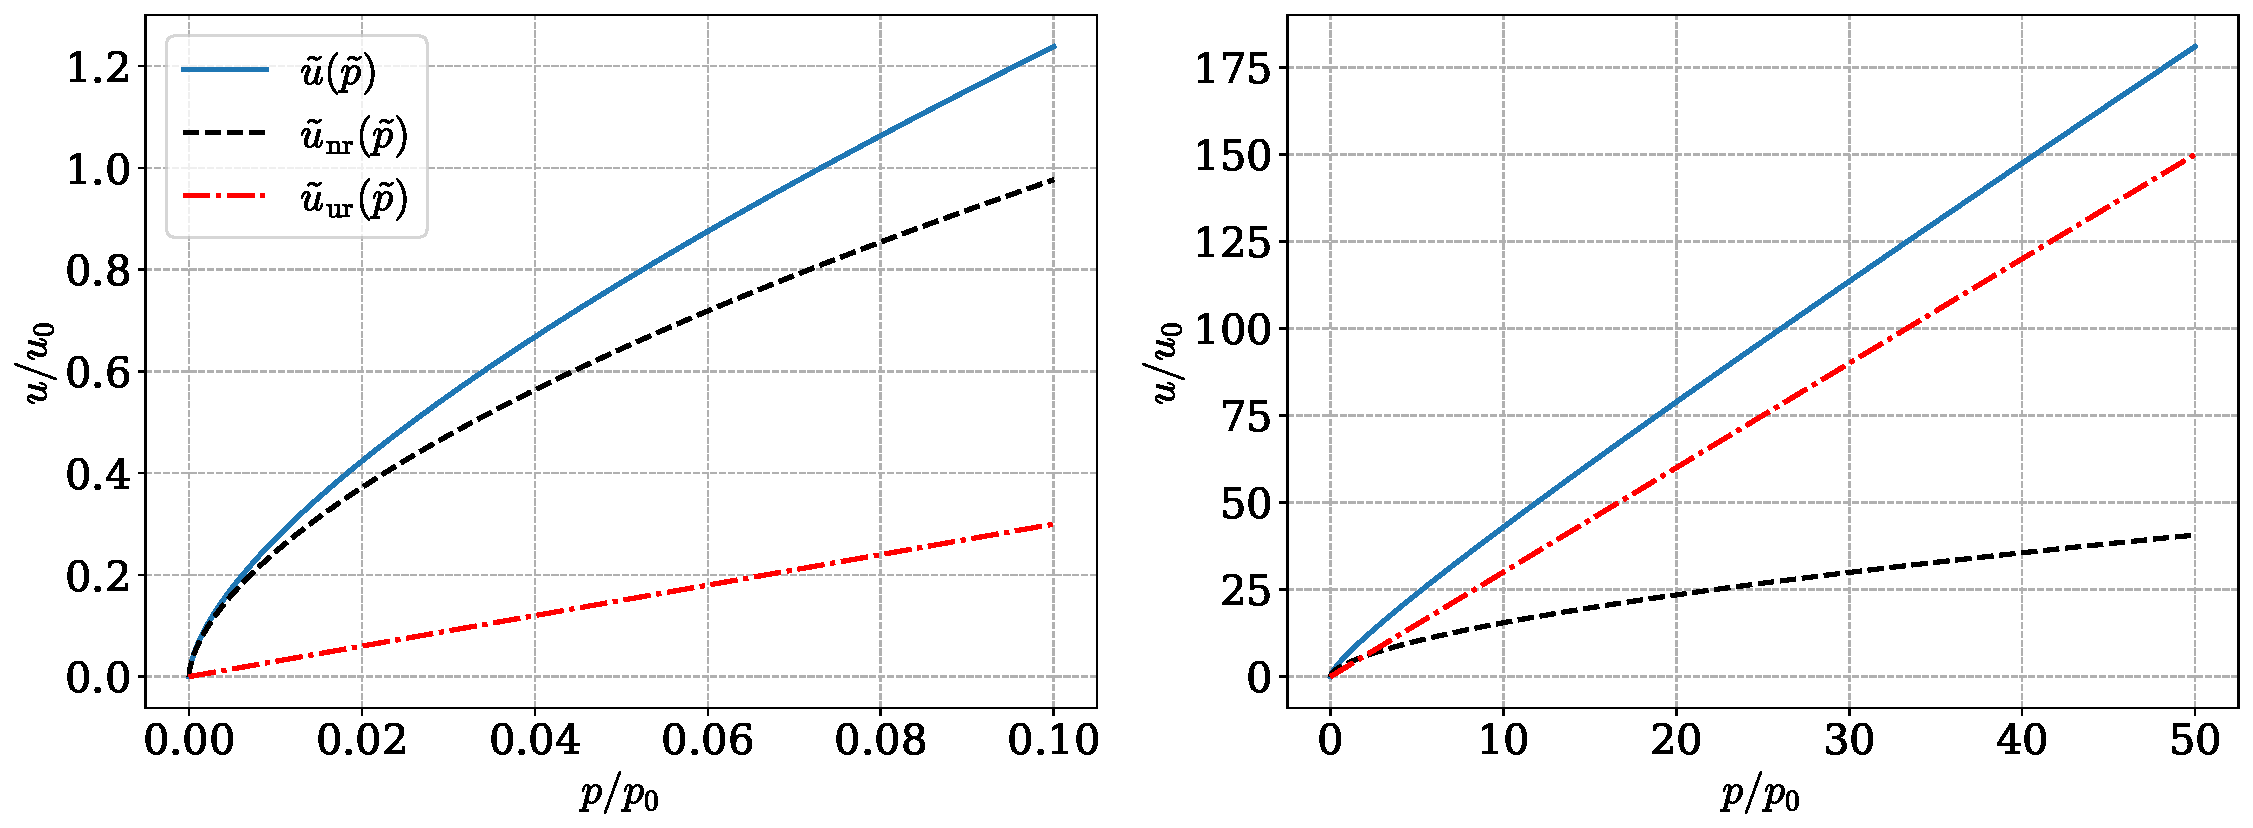
\includegraphics[width=\textwidth]{../scripts/figurer/fermi_eos.pdf}
    \caption{The equation of state of a cold Fermi gas. Both pressure and energy density is normalized to their characteristic quantities, $p_0$ and $u_0$. The equation of state is compared to the non-relativistic approximation, $\tilde u_{\mathrm{nr}}$ as well as the ultrarelativistic approximation, $\tilde u_{\mathrm{ur}}$, in two different regimes.}
    \label{fig: equation of state fermi fluid}
\end{figure}




\subsection{Units}

The equation of state has given us the characteristic energy density and pressure, $u_0$ and $p_0$. 
If we demand
%
\begin{equation}
    G \frac{m_0}{r_0} = \frac{4 \pi }{3}\frac{r_0^3 u_0}{m_0} = 1,
\end{equation}
%
we have two equations and two unknowns, $m_0$ and $r_0$.
This thus defines a complete set of units.
We are using the cold Fermi-gas as a model for a neutron star, an the mass of the fermion $m$ is therefore the neutron mass, \autoref{mass of neutron}, $m_N = 1.674 \cdot 10^{-27} \, \text{kg}$.
After reinstating $\hbar$ and $c$ in metric units, we get
%
\begin{align}
    u_0 &= p_0 = \frac{m^4}{8 \pi^2}\frac{c^5}{\hbar^3} 
    = 2.056\cdot10^{35}  \, \text{J}\,\text{m}^{-3}, \\
    m_0 &= \frac{c^4}{\sqrt{\frac{4 \pi}{3} u_0 G^3} }
    = 1.598 \cdot 10^{31} \, \text{kg}
    = 8.032 \, M_\odot, \\
    r_0 &= \frac{G m_0}{c^2} = 11.86 \, \text{km}. % sjekk
\end{align}
%
From this, we expect our star to have a mass of the order of a solar mass $M_\odot$ and a radius of the order of kilometers, without solving the TOV equation.




\subsection{Numerical results}



With the energy density, \autoref{Fermi gas energy density}, and pressure, \autoref{Fermi gas pressure}, we can numerically solve the TOV equation given a central pressure $p_c$. 
This is done using an adaptive Runge-Kutta method, with the stop criterion $p(r) = 0$.
Description of the code and where to find it is given in \autoref{appendix: code}.
The top graph in \autoref{fig: pressure and mass as a function of radius} shows the pressure, normalized to the central pressure $p_c$, as a function of radius, normalized to the corresponding stellar radius $R$.
The boundary conditions are logarithmically spaced.
The lower graph in \autoref{fig: pressure and mass as a function of radius} shows the mass, normalized to the total mass $M = m(R)$, as a function of the radius, again normalized to the stellar radius.
As in the case of an incompressible fluid, the pressure follows a half bell-shaped curve, with a peak that becomes narrower as the central pressure increases.
The black dashed line corresponds to the solution with the maximum mass, which will discuss shortly.
We see that the pressure and mass curves change most drastically when the central pressure is higher than that corresponding to the most massive star.

In \autoref{fig: mass radius relationship fermi gas}, we see the relationship between the mass and radius of the star.
This line is parametrized by the base-10 logarithm of the central pressure, $p(0)$, normalized by $p_0 = u_0$.
The cross marks the maximum mass, $M_\mathrm{max} = 0.711 \, M_\odot$, which corresponds to a radius of $R = 9.20 \, \mathrm{km}$.
This matches the results obtained by Oppenheimer and Volkoff~\cite{oppenheimerMassiveNeutronCores1939}, $M_\mathrm{max} = 0.71$.
In their 1939 paper, Oppenheimer and Volkoff computed five data points in the mass-radius plane.
The results are marked by blue circles in \autoref{fig: mass radius relationship fermi gas}.
We find good agreement between the three points closest to the maximum value and our results.
However, the two results of Oppenheimer and Volkoff furthest away differ significantly from our results.
The black dashed line is the absolute mass-radius constraint, \autoref{mass radius constraint}, and any stable configuration must be on the right side of this line.
As we predicted from looking at the non-relativistic equation of state, the mass decreases with the star's radius, at least for stars with low central pressure.

In \autoref{fig: mass radius relationship comparison}, we compare the mass-radius relationship obtained from the full theory with results from approximations.
The lowest line is obtained by using both the full TOV equation and the exact equation of state.
The next line above is obtained using the non-relativistic equation of state together with the full TOV equation.
The second uppermost line is obtained from the exact equation of state and the Newtonian approximation for the TOV equation.
The uppermost line uses both the Newtonian approximation to the TOV equation and the non-relativistic approximation for the equation of state.
This last line corresponds to a polytrope in Newtonian gravity, as we studied in \autoref{subsection: Newtonian limit and polytropes}.
Unlike the other systems, it does not seem to have an upper limit for the mass, as expected.
\vfill

\begin{figure}[h]
    \centering
    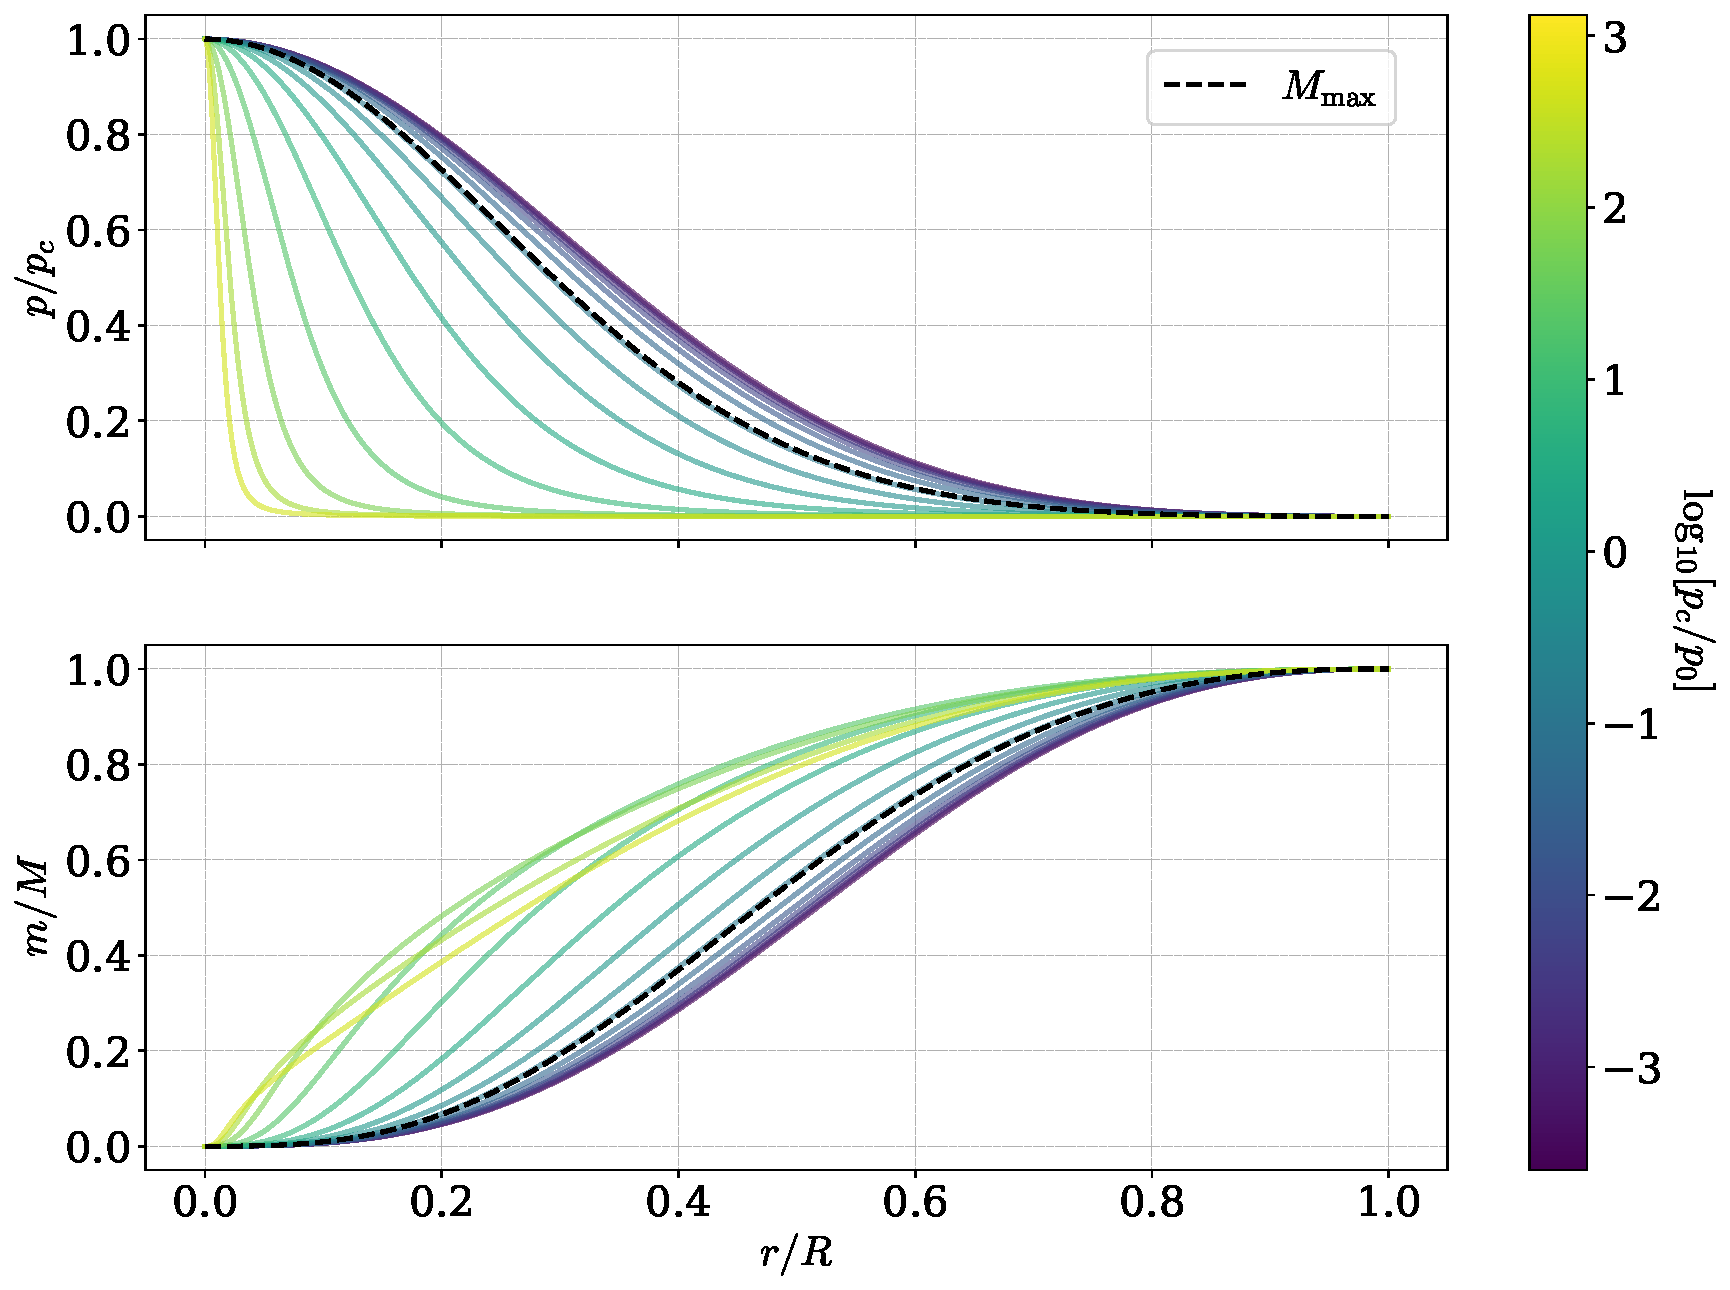
\includegraphics[width=\textwidth]{../scripts/figurer/pressure_mass.pdf}
    \caption{
        Top: The pressure normalized to central value, as a function of radius, normalized to the stellar radius.
        Bottom: The mass normalized to the total mass, as a function of radius, normalized to the stellar radius. 
        This is plotted for several different values of central pressure, which is indicated by the color scheme.
        }
    \label{fig: pressure and mass as a function of radius}
\end{figure}


\begin{figure}[p]
    \centering
    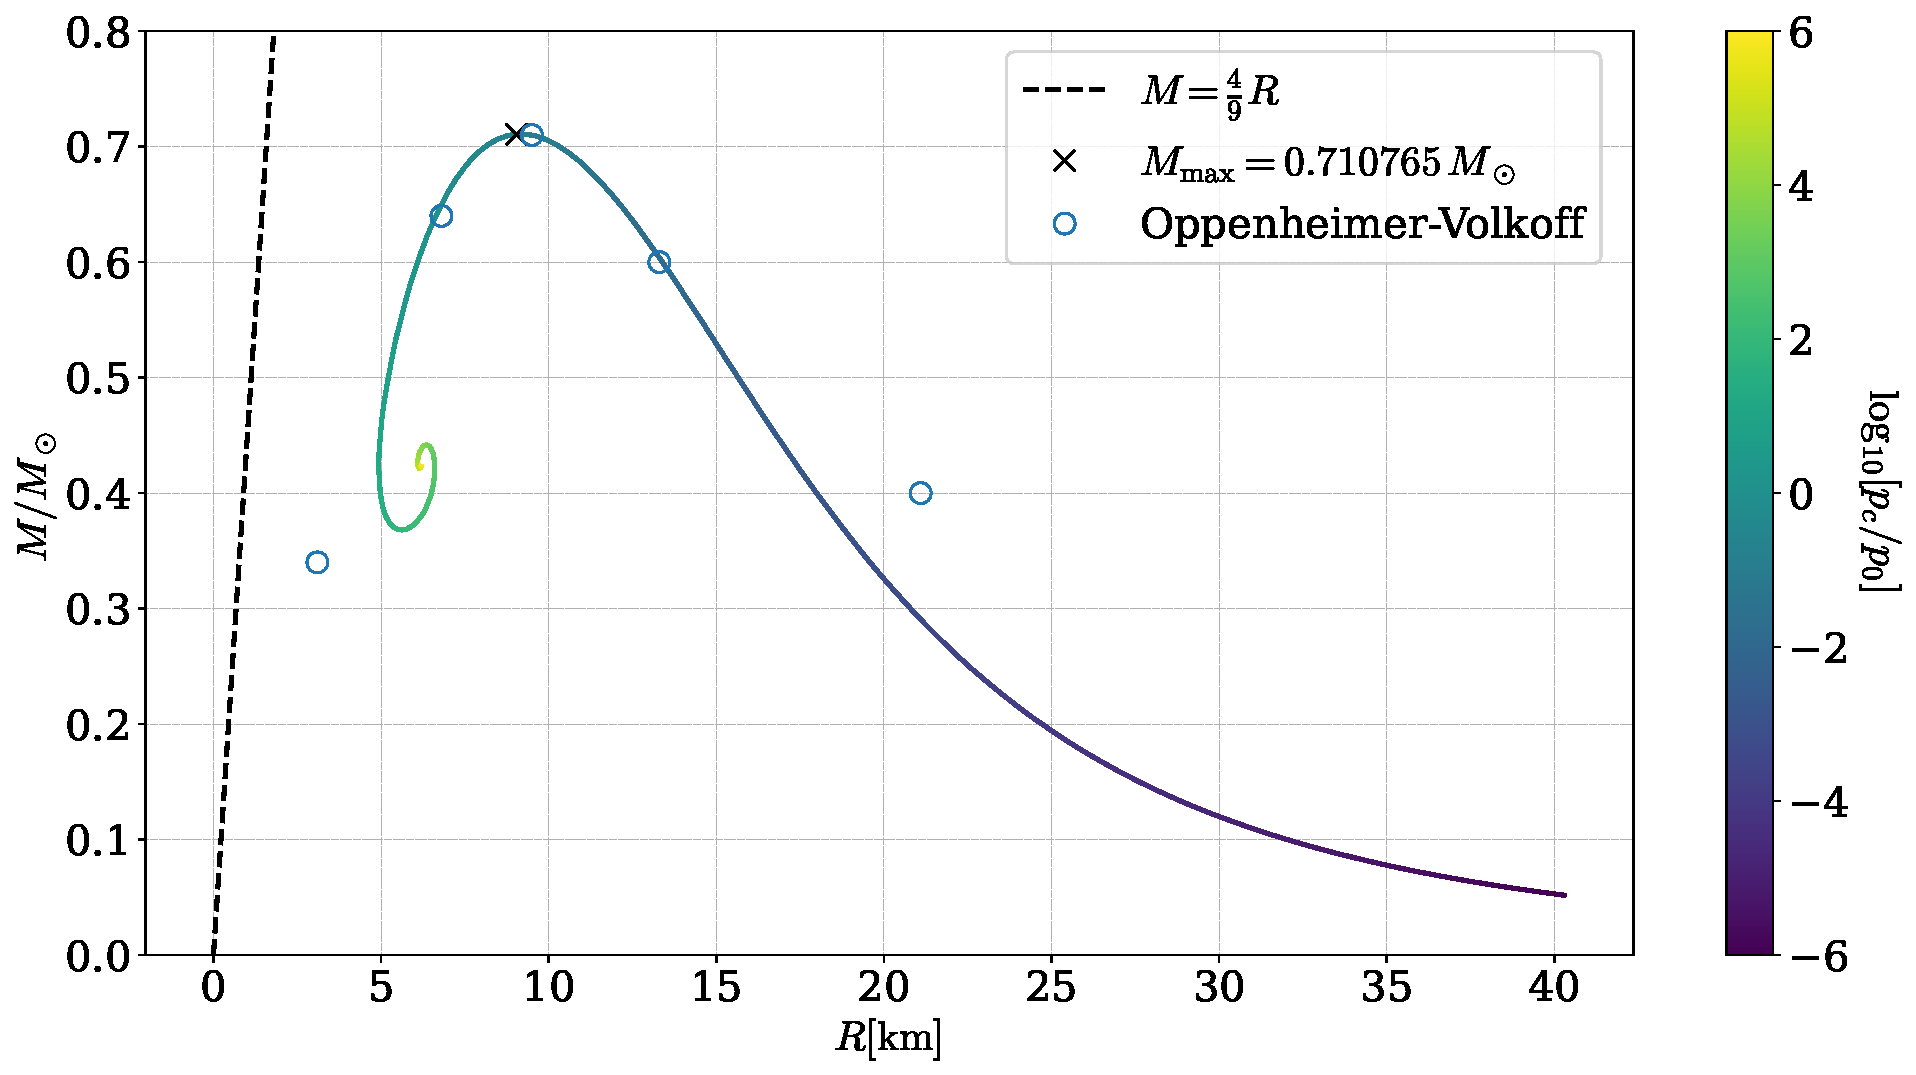
\includegraphics[width=\textwidth]{../scripts/figurer/mass_radius_neutron.pdf}
    \caption{The mass-radius relationship of a star made of a cold gas of neutrons. The line is parametrized by the central pressure $p_c$. The corss indicate the maximum mass solution. The blue circles are results form the 1939 paper of Oppenheimer and Volkoff~\autocite{oppenheimerMassiveNeutronCores1939}.}
    \label{fig: mass radius relationship fermi gas}
\end{figure}

\begin{figure}[p]
    \centering
    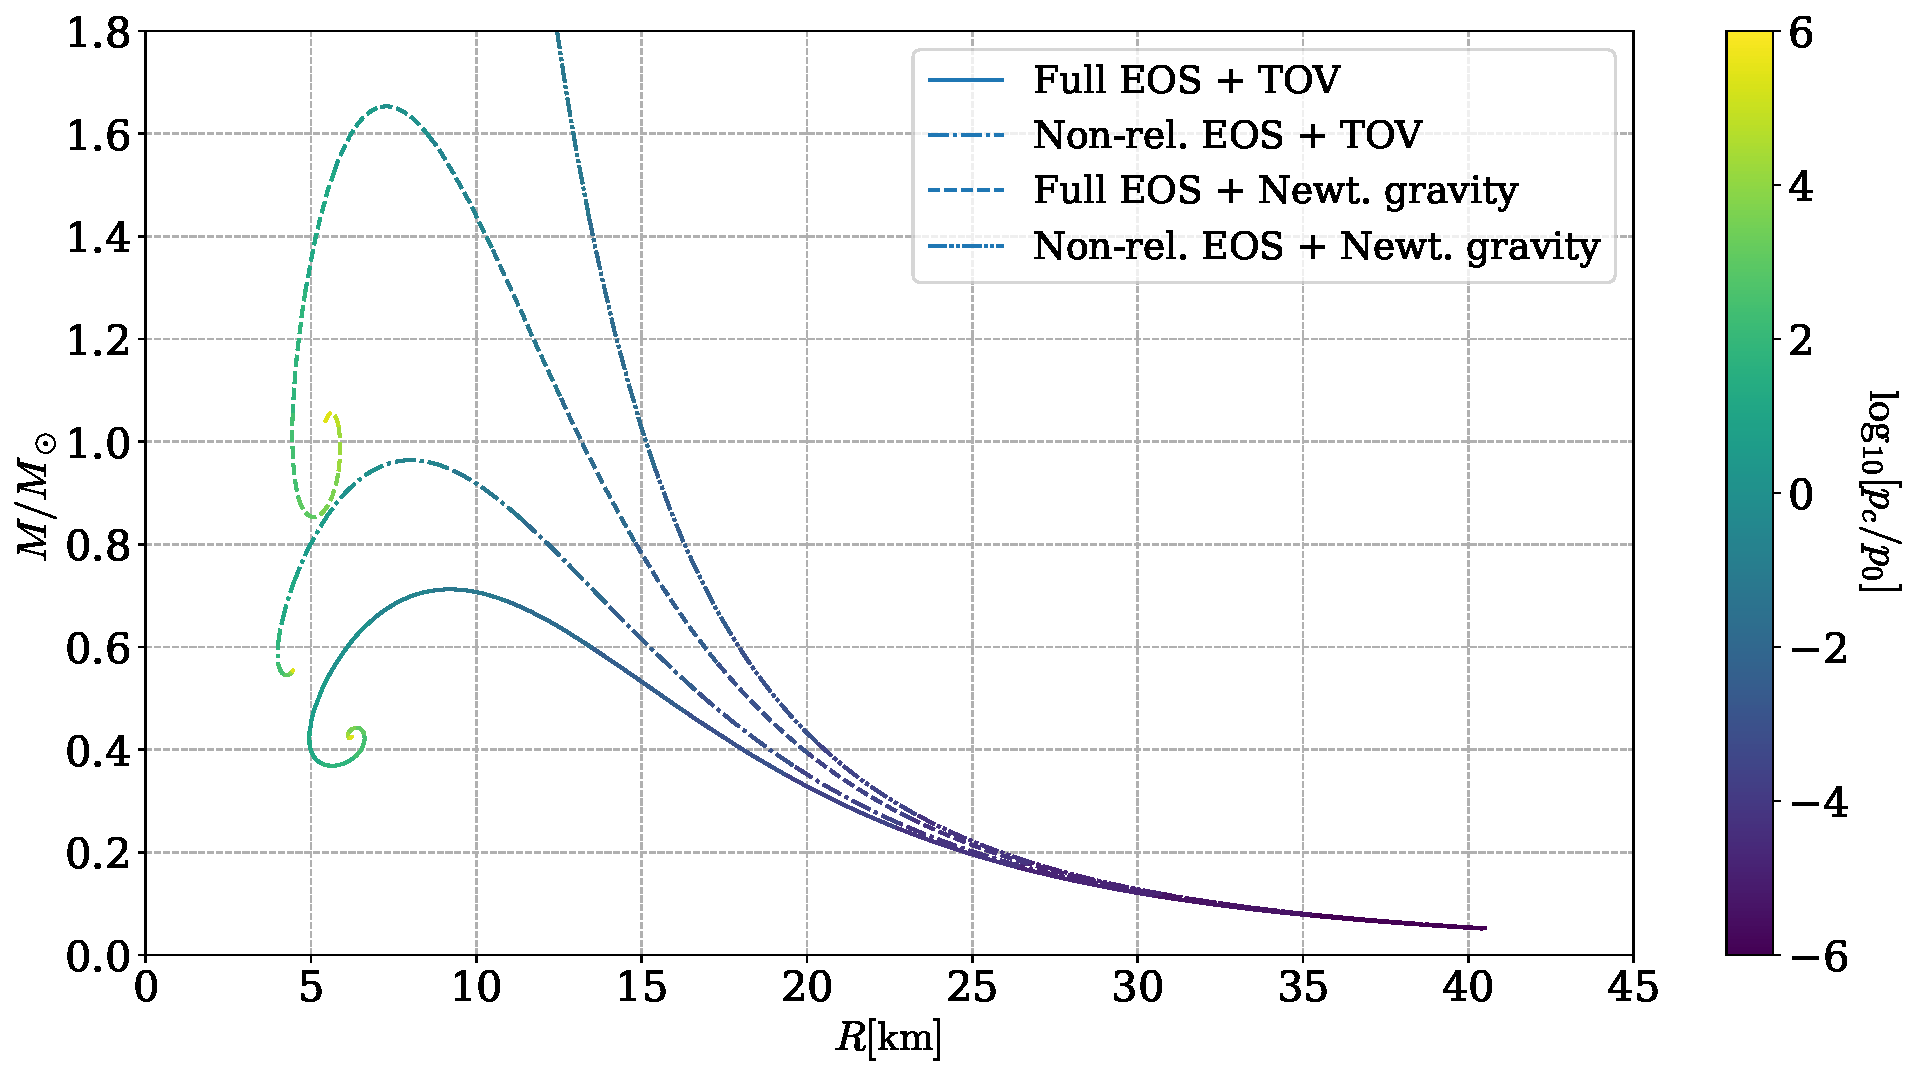
\includegraphics[width=\textwidth]{../scripts/figurer/mass_radius_comparison.pdf}
    \caption{The mass-radius relationship of a cold gas of neutrons. The lowest line is obtained from the TOV equation and full equation of state. The middle line is from the TOV equation and the non-relativistic equation of state. The upper line is obtained from the Newtonian approximation of the TOV equation and the non-relativistic equation of state.}
    \label{fig: mass radius relationship comparison}
\end{figure}

\FloatBarrier



\subsection{Upper bound and stability}
\label{subsection: upper bound and stability}


For any equation of state, the TOV equation will give a one-parameter family of stars, parametrized by the central pressure $p_c$~\autocite{misnerGravitation2009}.
This leads to the possibility of an \emph{absolute maximum} mass for a given equation of state.
In the case of a non-interacting neutron, we found the limit to be $0.71 \, M_\odot$, in agreement with Oppenheimer and Volkoff~\autocite{oppenheimerMassiveNeutronCores1939}.
To obtain a more general upper limit for the mass of neutron stars or other compact stars in, one has to account for more general equations of state.
To constrain the equation of state, we assume firstly that $\odv{p}/{u} \geq 0$.
To justify this, take the non-relativisitc case, $u = n$, in which case the assumption is equivalent to $\odv{p}/{n} \geq 0$.
This says that an increase in particle density, for example, due to compression, will result in a rise in pressure.
This is an instance of Le Chatelier's principle: nature will counteract any change forced upon it.
If we perturb a perfect fluid, then in its stationary frame we have $n = n_0 + \delta n$, $v^\mu = (1, \delta v^i)$, $p = p_0 + \delta p$ and $u = u_0 + \delta u$.
Combining the conservation of energy, $\partial_\mu T^{\mu \nu} = 0$, and conservation of matter, $\partial_\mu (n v^\mu) = 0$, with the first law of thermodynamics, \autoref{firs law of thermodynamics fluid}, we can obtain a wave equation for the propagation of the perturbation,
%
\begin{equation}
    (\partial_t^2 - v_s^2 \nabla^2) \delta n = 0,
\end{equation}
%
where the speed of sound in the fluid, $v_s$, is given by~\autocite{weinbergGravitationCosmologyPrinciples1972}
%
\begin{equation}
    v_s^2 = \odv{p}{u}.
\end{equation}
%
A realistic fluid should not have a speed of sound greater than the speed of light, leading to the constraint $\odv{p}/{u} < 1$.
Using these general assumptions, Rhoades and Ruffini found an upper limit for neutron stars of $3.2 \, M_\odot$~\cite{rhoadesMaximumMassNeutron1974}.

An equation of state with a \emph{high} speed of sound, i.e., with a flat curve in the $p-u$-plane, is called \emph{stiff}.
From \autoref{fig: equation of state fermi fluid}, we see that the Newtonian equation of state is stiffer in the high-energy regime.
The most extreme case is the incompressible model we saw earlier, which breaks causality.
In general, a stiffer equation of state leads to a larger maximum mass.
This is intuitive; the TOV equation describes the balancing of forces from pressure and gravity, and if the pressure raises fast as the density increases, then it can sustain a large total mass before it collapses~\autocite{glendenningCompactStarsNuclear2012}.


Solutions to the TOV equation are systems in hydrostatic equilibrium.
However, as a pen perfectly balances on its edge, equilibrium does not imply stability.
When perturbed, a stable system returns to its equilibrium position as a marble at the bottom of a bowl.
On the other hand, an unstable system will amplify perturbations, leading to a collapse or an explosion.
We can make an intuitive argument for which configurations for a given family of stars are stable.
We will again assume that the equation of state, on a microscopic level, obeys Le Chatelier's principle in the form $\odv{p}/{n} > 0$.
We can see that this holds for all the cases we are considering.
A star in equilibrium will find itself on the line parametrized by its central pressure, such as \autoref{fig: mass radius relationship fermi gas}.
In this case, a perturbation reducing the radius of the star will increase the central pressure as the particle density increases.
This is illustrated in \autoref{fig: fermi stability}.
A star in equilibrium at point A can be compressed to an out-of-equilibrium configuration, point B.
This point has a central pressure corresponding to the equilibrium state at point C.
As the equilibrium configuration at point C has a \emph{lower} mass than the configuration at B, it has a weaker gravitational effect.
Therefore, we would expect it to shrink further, as the central pressure of B is not enough to support its gravitational mass.
This compression will lead to an even higher central pressure.
We thus have a positive feedback loop, and the initial perturbation will continue to grow.
We can make a similar argument in the case where the mass increases with an increase in the central pressure.
Here, a compression will lead to a state in which central pressure corresponds to an equilibrium state with a \emph{higher} mass.
This state will thus tend to expand after a compression, counteracting the perturbation.
This gives us the following criterion for stability,
%
\begin{equation}
    \odv{M}{p_c} > 0.
\end{equation}

\begin{figure}[!h]
    \centering
    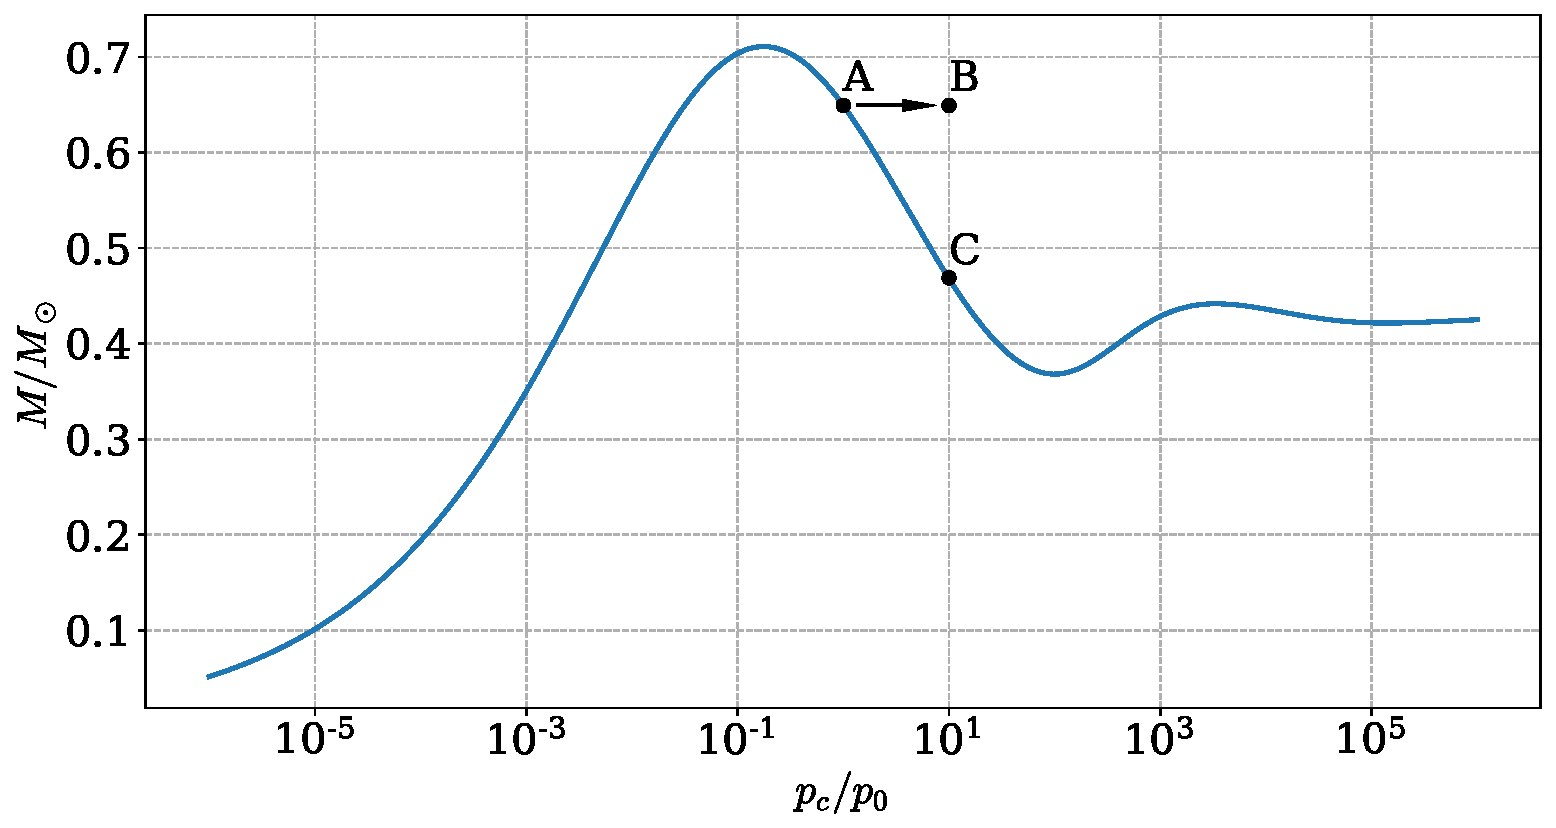
\includegraphics[width=0.7\textwidth]{../scripts/figurer/fermi_stability.pdf}
    \caption{
        The plot shows the mass, in units of solar masses, of a star of a cold gas of neutrons, as a function of the central pressure, normalized to the characteristic pressure.
    Point A denotes a position of equilibrium, which can be compressed to an out-of-equilibrium point, B, which has a central pressure corresponding to an equilibrium configuration, point C.
    }
    \label{fig: fermi stability}
\end{figure}

As it turns out, this is a necessary but not sufficient requirement for stability~\autocite{glendenningCompactStarsNuclear2012}.
To conduct a more rigorous study of stability, one must derive the equation of hydrostatic equilibrium with the addition of perturbations as time-dependent, radial oscillations.
This is beyond the scope of this thesis, but we shortly recap the  procedure.
This is done by discplacing a fluid elemet at a radius $r$ and time $t$ by $\delta r(r, t) = \sum_n A_n \xi_n(r) e^{i \omega_n t}$.
Here, $\xi_n$ are normal modes with frequencies $\omega_n$, $n \in \{0, 1, ...\}$.
The equation for the eigenmodes was first obtained by Chandrasekhar~\autocite{chandrasekharDynamicalInstabilityGaseous1964}, and can be written in the form of a Sturm-Liouville theory equation,
%
\begin{equation}
    \left[     \odv{}{r} \left( \Pi \odv{}{r}  \right) + Q + \omega_n W \right] \xi_n
    = 0,
\end{equation}
%
where $\Pi$, $Q$, and $W$ are functions of the pressure, energy density, particle density, $\alpha$, and $\beta$.
These quantities are thus given by a solution to the equilibrium problem~\cite{glendenningCompactStarsNuclear2012}.
Stability is encoded in the sign of the square of the frequencies.
For $\omega_n^2>0$, the mode will remain oscillatory, while if $\omega_n^2<0$, it will grow exponentially.
Thus, if the system has \emph{any} modes such that $\omega_n^2<0$, it is unstable.
One mode $\omega_n$ will change stability at a critical point on the $M-R$ curve, where
%
\begin{equation}
    \odv{M}{u_c} = 0,
\end{equation}
%
and this will \emph{only} happen at critical points~\autocite{thorneGeneralRelativisticTheoryStellar1968}. Here, $u_c$ is the central energy density corresponding to $p_c$.
This is equivaent to the criterion $\odv{M}/{p_c} = 0$ as long as $\odv{p}/{u}$ is finite.
Whether the change is from a stable mode to an unstable one is dependent on whether the curve turns clockwise (a mode becomes stable) or counterclockwise (a node becomes unstable)~\autocite{thorneGeneralRelativisticTheoryStellar1968}.
We know that very low-pressure, cold fermions are stable, which means that configuration with a radius larger than the maximum mas $0.71 \, M_\odot$ will be stable.
As illustrated in \autoref{fig: mass radius relationship fermi gas}, the curve then turns counterclockwise, and a new mode is made unstable each half turn.
